\documentclass[12pt]{article}
\usepackage{amsmath}
\usepackage{amssymb}
\usepackage{geometry}
\usepackage{enumerate}
\usepackage{natbib}
\usepackage{float}%稳定图片位置
\usepackage{graphicx}%画图
\usepackage[english]{babel}
\usepackage{a4wide}
\usepackage{indentfirst}%缩进
\usepackage{enumerate}%加序号
\usepackage{multirow}%合并行
\title{\large UM-SJTU JOINT INSTITUTE\\Intro to Circuits\\(VE215)\\\ \\\ \\\ \\\ \\\ \\\ \\\ \\\ \\\ \\\ \\\
LABORATORY REPORT\\\ \\\ EXERCISE 2\\\ OP Amp Lab \\\ \\\ \\\ \\\ \\\ }
\author{Name: Pan Chongdan\\ID: 516370910121\\Group: 16}
\date{Date: \today}
\begin{document}
\maketitle
\newpage
\section{Introduction and Theoretical Background}
\subsection{Objectives}
\begin{enumerate}
\item Learn how to build and test a variety of circuits based on LM 741 Op Amp chip: non-inverting and inverting amplifiers with fixed gain.
\item Measure the gain of the amplifier and compare it with theoretical calculations.
\item Determine the saturated output voltage of the amplifier.
\end{enumerate}
\subsection{Introduction}
Operational amplifiers are integrated circuits used in many applications and I built and studied LM741.
\subsubsection{Op Amp Terminals}
\begin{figure}[H]
\centering
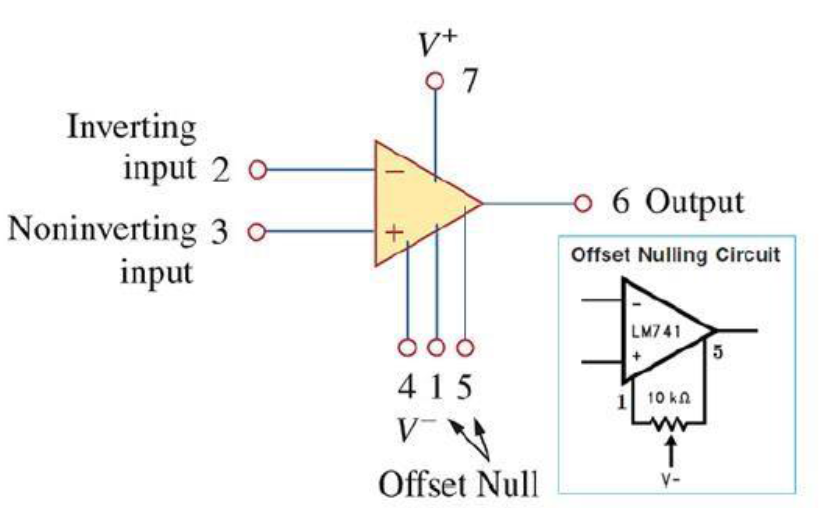
\includegraphics[scale=0.5]{P1.jpg}
\caption{Circuit symbol of a typical op amp}
\end{figure}
In Figure 1, there are :
\begin{enumerate}
\item Two terminals for input signals: inverting (labeled -) and non-inverting (labeled +)
\item A terminal for the output signal
\item Two terminals for the power supply voltages: positive +Vcc and negative –Vcc.
\end{enumerate}
Figure 2 shows the pin numbers of LM741
\begin{figure}[H]
\centering
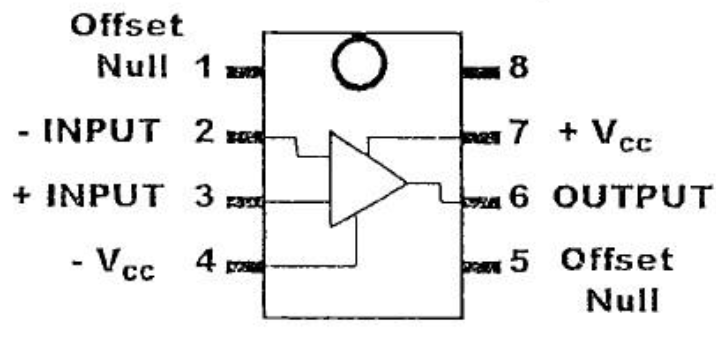
\includegraphics[scale=0.5]{P2.jpg}
\caption{Pin numbers for LM 741 op amp Note:}
\end{figure}
\begin{enumerate}
\item Pin 8 is not connected; pins 1 and 5 are not used in this lab.
\item Do not mistake the connections of input signals 2 labeled – and 3 labeled +) for the connections to the power supply (4 for -Vcc and 7 for +Vcc).
\item Make sure you connect the grounds of oscilloscope, function generator and DC source together.
\end{enumerate}
\subsubsection{The Gain of Amplifier Circuits}
The amplifier circuits are characterized by their gain values. The voltage gain
is the ratio of output voltage to the input voltage in the circuit:
$$Voltage Gain=\frac{OutputVoltage}{InputVoltage}$$
In the lab, you can use oscilloscope to measure the input and output
peak-to-peak amplitudes of the signals through two channels at the same
time.
\subsubsection{Inverting amplifier}
\begin{figure}[H]
\centering
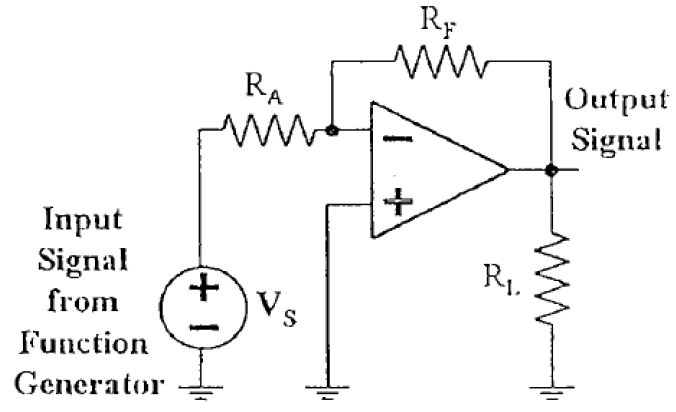
\includegraphics[scale=0.3]{P3.jpg}
\caption{Inverting Amplifier}
\end{figure}
For inverting amplifier, the theoretical gain should be:
$$Gain=\frac{V_{out}}{V_s}=-\frac{R_F}{R_A}$$
\subsubsection{Non-inverting Amplifier}
\begin{figure}[H]
\centering
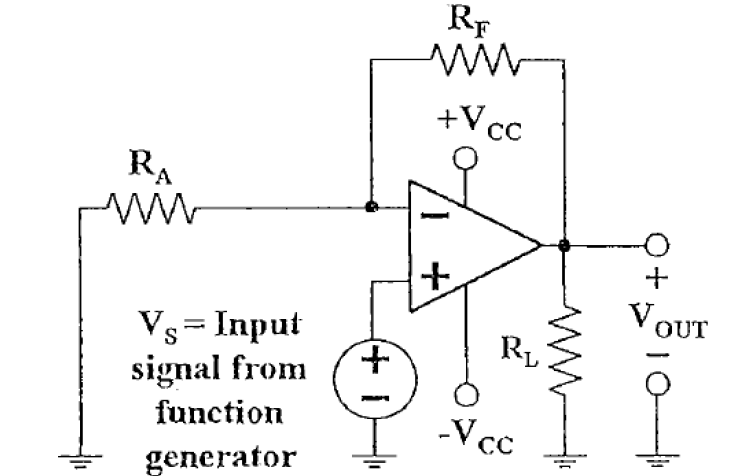
\includegraphics[scale=0.3]{P4.jpg}
\caption{Inverting Amplifier}
\end{figure}
For non-inverting amplifier, the theoretical gain should be:
$$Gain=\frac{V_{output}}{V_S}=1+\frac{R_F}{R_A}$$
\section{Apparatus}
I used function generator and oscilloscope in exercise 2.
\subsection{Function Generator}
\begin{figure}[H]
\centering
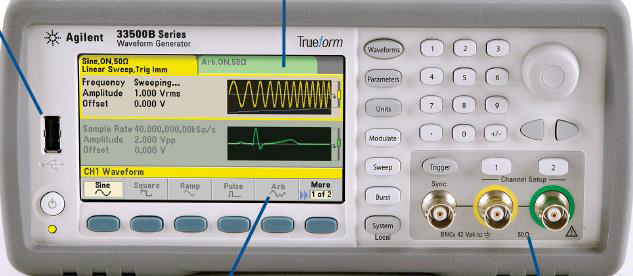
\includegraphics[scale=0.3]{P5.jpg}
\caption{Function Generator}
\end{figure}
\begin{enumerate}
\item "Parameter": to change the amplitude, frequency of wave to generate. The amplitude here equals to half of the pp value.
\item “1”/ 2”: to switch on the channel.
\end{enumerate}
\subsection{Oscilloscope}
\begin{figure}[H]
\centering
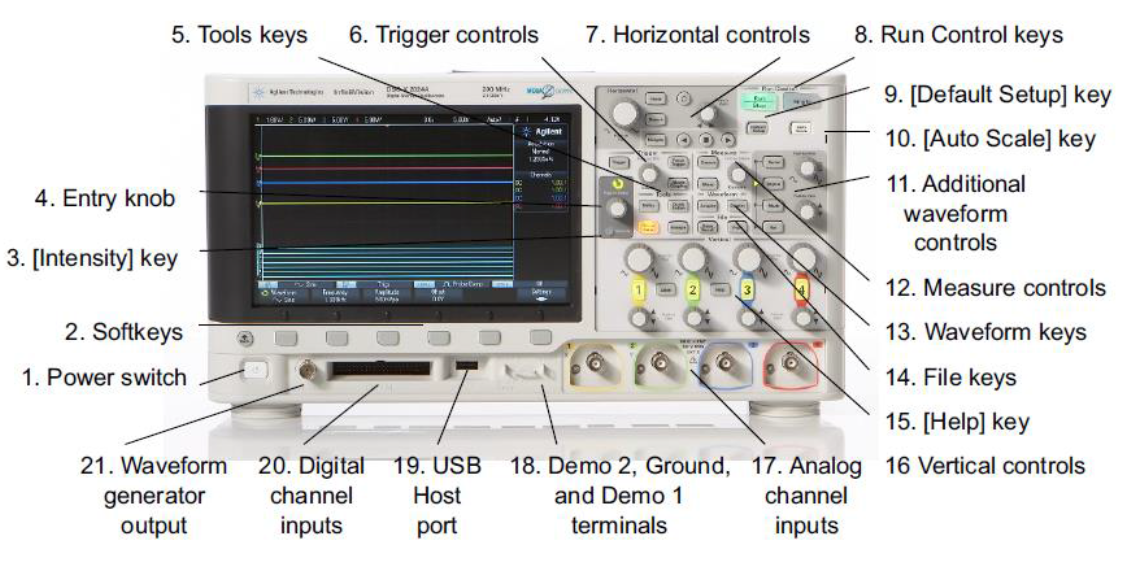
\includegraphics[scale=0.3]{P6.jpg}
\caption{Oscilloscope}
\end{figure}
\begin{enumerate}
\item “Auto scale”: to automatically achieve an output on the screen with proper scale.
\item "Means": to turn on the measurement of the wave.
\item "1"$\setminus$"2": to show or hide the wave you detecting through channel 1 or 2.
\end{enumerate}
\section{Results}
\subsection{Non-inverting Amplifier}
\subsubsection{The resistances of the two resistors we used to build the circuit.}
\begin{table}[H]
\centering
\begin{tabular}{|c|c|}
\hline
$R_1[\Omega]$        &51.3      \\ \hline
$R_f[\Omega]$        &99.5    \\ \hline
\end{tabular}
\end{table}
\subsubsection{The voltage supplied to the op amp.}
\begin{table}[H]
\centering
\begin{tabular}{|c|c|}
\hline
$+V_{cc}[V]$       &+5      \\ \hline
$-V_{cc}[V]$        &-5    \\ \hline
\end{tabular}
\end{table}
\subsection{The input/output relationship}
\begin{table}[H]
\centering
\begin{tabular}{|c|c|c|}
\hline
$V_{PP(in)}$[V]    &$V_{PP(out)}$[V] &Gain   \\ \hline
0.2 &$33.4\times 10^{-3}$&0.167  \\ \hline
0.4 &$62.3\times 10^{-3}$&0.156  \\ \hline
0.6 &$90.5\times 10^{-3}$&0.151  \\ \hline
0.8 &$121\times 10^{-3}$&0.152  \\ \hline
1.0 &$0.15$&0.150  \\ \hline
1.2 &$0.179$&0.149  \\ \hline
1.4 &$0.211$&0.151  \\ \hline
1.6 &$0.243$&0.152  \\ \hline
1.8 &$0.271$&0.151  \\ \hline
2.0 &$0.300$&0.150 \\ \hline
2.2 &$0.332$&0.151  \\ \hline
2.4 &$0.352$&0.147  \\ \hline
2.6 &$0.368$&0.142  \\ \hline
2.8 &$0.382$&0.137  \\ \hline
3.0 &$0.396$&0.132  \\ \hline
3.2 &$0.402$&0.126  \\ \hline
3.4 &$0.402$&0.118	  \\ \hline
\end{tabular}
\end{table}
\subsection{Inverting Amplifier}
\subsubsection{The resistances of the two resistors we used to build the circuit.}
\begin{table}[H]
\centering
\begin{tabular}{|c|c|}
\hline
$R_1[\Omega]$        &51.3      \\ \hline
$R_f[\Omega]$        &99.5    \\ \hline
\end{tabular}
\end{table}
\subsubsection{The voltage supplied to the op amp.}
\begin{table}[H]
\centering
\begin{tabular}{|c|c|}
\hline
$+V_{cc}[V]$       &+5      \\ \hline
$-V_{cc}[V]$        &-5    \\ \hline
\end{tabular}
\end{table}
\subsection{The input/output relationship}
\begin{table}[H]
\centering
\begin{tabular}{|c|c|c|}
\hline
$V_{PP(in)}$[V]    &$V_{PP(out)}$[V] &Gain   \\ \hline
0.2 &$22.1\times 10^{-3}$&0.111  \\ \hline
0.4 &$41.8\times 10^{-3}$&0.105  \\ \hline
0.6 &$60.3\times 10^{-3}$&0.101  \\ \hline
0.8 &$78.4\times 10^{-3}$&0.098  \\ \hline
1.0 &$96.5\times 10^{-3}$&0.097  \\ \hline
1.2 &$0.112$&0.094  \\ \hline
1.4 &$0.129$&0.092  \\ \hline
1.6 &$0.147$&0.092  \\ \hline
1.8 &$0.166$&0.092  \\ \hline
2.0 &$0.183$&0.092 \\ \hline
2.2 &$0.203$&0.093  \\ \hline
2.4 &$0.221$&0.092 \\ \hline
2.6 &$0.241$&0.093  \\ \hline
2.8 &$0.259$&0.093  \\ \hline
3.0 &$0.271$&0.091  \\ \hline
3.2 &$0.283$&0.086  \\ \hline
3.4 &$0.289$&0.085	  \\ \hline
3.6 &$0.297$&0.083  \\ \hline
3.8&$0.304$&0.080 \\ \hline
4.0 &$0.304$&0.076	  \\ \hline
\end{tabular}
\end{table}
\section{Discussion}
\subsection{Relation between $V_{pp(out)}$ vs. $V_{pp(in)}$}
\subsubsection{Non-inverting Amplifier}
$$V_1=V_{pp(in)}$$
$$\frac{0-V_1}{R_A}=\frac{V_1-V_{pp(out)}}{R_f}$$
$$Gain=\frac{V_{pp(out)}}{V_{pp(in)}}=1+\frac{R_f}{R_A}$$
\begin{figure}[H]
\centering
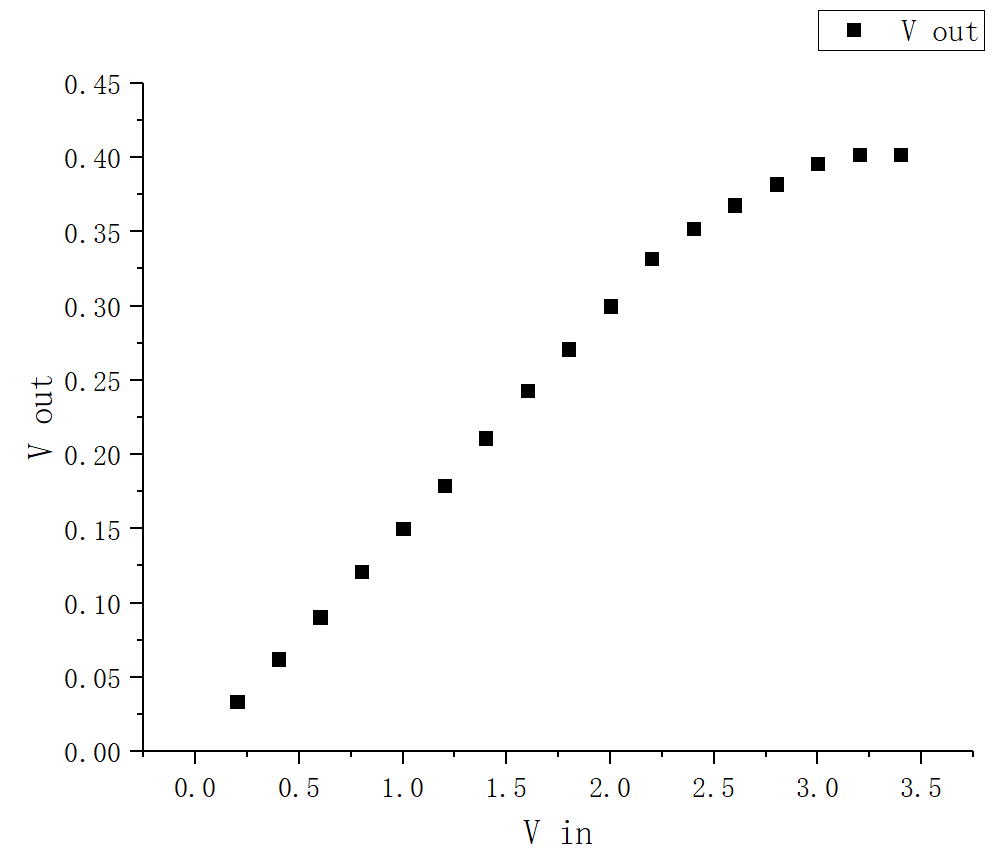
\includegraphics[scale=0.3]{P7.jpg}
\caption{Relation between $V_{pp(out)}$ the $V_{pp(in)}$ for non-inverting amplifier}
\end{figure}
\subsubsection{Inverting Amplifier}
$$\frac{V_{pp(in)}}{R_A}=\frac{0-V_{pp(out)}}{R_f}$$
$$Gain=\frac{V_{pp(out)}}{V_{pp(in)}}=-\frac{R_f}{R_A}$$
\begin{figure}[H]
\centering
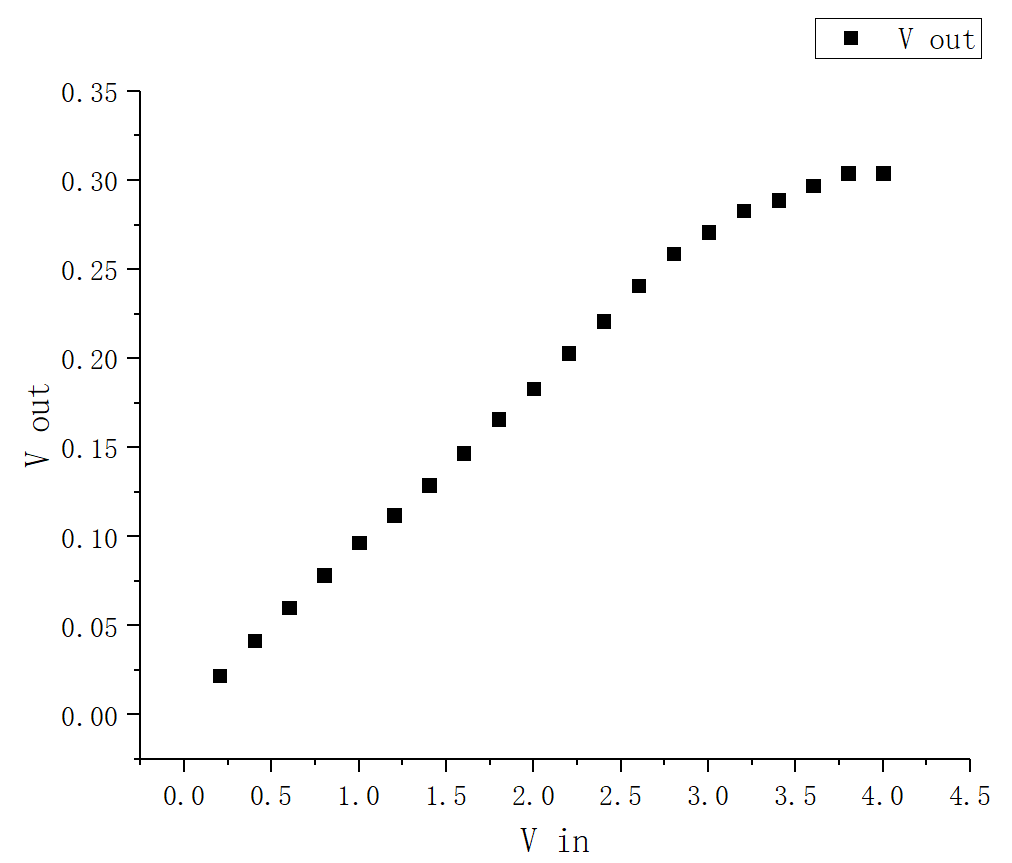
\includegraphics[scale=0.3]{P8.jpg}
\caption{Relation between $V_{pp(out)}$ the $V_{pp(in)}$ for inverting amplifier}
\end{figure}
\subsection{Calculation, Uncertainty Analysis, and Plot}
\subsubsection{Non-inverting Amplifier}
$$\bar{Gain}=\frac{1}{17}\sum^{17}_{i=1}Gain_i=0.146$$
$$s_X=0.012$$
$$u=0.012/0.5=0.024$$
$$u_r=16.44\%$$
$$Gain=0.146\pm0.024$$
\begin{figure}[H]
\centering
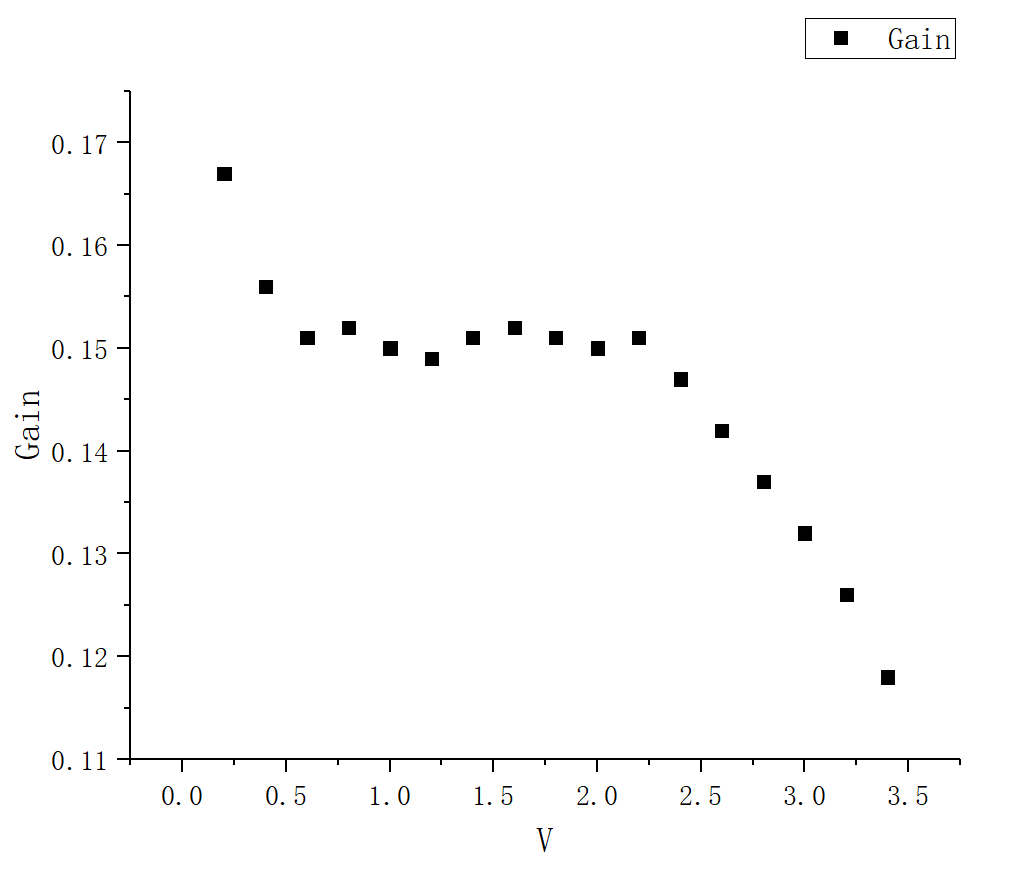
\includegraphics[scale=0.3]{P9.jpg}
\caption{Relation between gain the $V_{pp(in)}$ for non-inverting amplifier}
\end{figure}
\subsubsection{Inverting Amplifier}
$$\bar{Gain}=\frac{1}{20}\sum^{20}_{i=1}Gain_i=0.092$$
$$s_X=8.09\times10^{-3}$$
$$u=8.09\times10^{-3}/0.467=0.017$$
$$u_r=18.47\%$$
$$Gain=0.092\pm0.017$$
\begin{figure}[H]
\centering
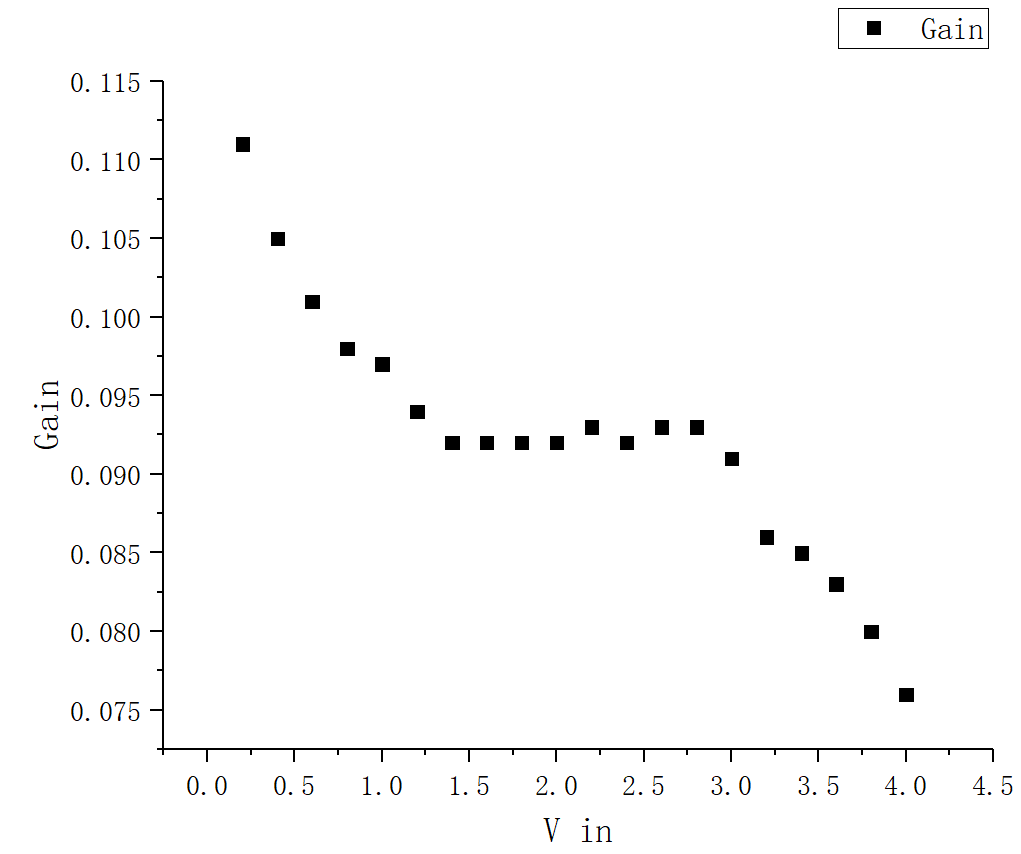
\includegraphics[scale=0.4]{P10.jpg}
\caption{Relation between gain the $V_{pp(in)}$ for non-inverting amplifier}
\end{figure}
\subsection{Error Analysis}
For non-inverting amplifier,the theoretical gain =$1+\frac{99.5}{51.3}=2.93$,but my data is 0.146. For inverting amplifier, theoretical gain =-1.94 while my data is 0.092. All my data is about 5\% of the theoretical gain, I think it's because my function generator's output voltage reading is wrong. Because if there exists a resistor of big resistance, the ration of the theoretical gain of measured gain shouldn't be same. 
\par I find two potential reasons causing the error in the output voltage reading. The first reason is the oscilloscope's vertical scale and the probe is set wrong. The second reason is the oscilloscope may present the $V_{pp}$ higher than the function generator. The root cause is the generator doesn't generates a function that the oscilloscope is expecting. In addition, I might make some mistake in reading the voltage such as choosing the wrong unit, etc.
\par The relative uncertainty is pretty high, I think there also two reasons. First, the amplifiers used are not ideal, they have their own resistance, which will cause the error. Second, the points in my figure make up a line approaching lever when $V_{in}$ is becoming bigger, it's because the amplifier is saturated and $V_{out}$ wont' be bigger after that. For an ideal amplifier, the line should be straight. 
\par In later lab work, I should be more carefully about the unit of all physical quantities as well as pay more attention to the amplification factor of the oscilloscope to make sure the oscilloscope match the function generator.
\section{Reference}
\begin{enumerate}[-]
\item \emph{VE215FA2017 OP AMP LabManual} 
\item \emph{Circuits Make Sense}, Alexander Ganago, Department of Electrical Engineering and Computer Science, University of Michigan, Ann Arbor.
\end{enumerate}
\end{document}